\chapter{آشنایی با درس و وظایف پایین‌دستی (\eng{Downstream Tasks})}

\section{معرفی درس}

\subsection{پردازش گفتار و پردازش سیگنال دیجیتال}
درس «پردازش گفتار» با درس «پردازش سیگنال دیجیتال» (\eng{Digital Signal Processing - DSP}) تفاوت اساسی دارد. پردازش سیگنال حوزه‌ای بنیادی و گسترده است و در رادار، مخابرات، تبدیل فوریه و تحلیل انواع سیگنال‌ها کاربرد دارد. پردازش گفتار را می‌توان یکی از شاخه‌های تخصصی و کاربردی پردازش سیگنال دانست که بر \emph{گفتار انسان} متمرکز است.

\begin{table}[htbp]
\centering
\caption{مقایسهٔ رویکرد دو درس}
\begin{tabular}{p{3cm}p{10cm}}
\toprule
درس & رویکرد \\
\midrule
\eng{DSP} & بنیادی، سیگنالی و ریاضیاتی \\
پردازش گفتار & کاربردی و مبتنی بر هوش مصنوعی؛ تمرکز بر تحلیل، درک و تولید گفتار انسان \\
\bottomrule
\end{tabular}
\end{table}

ممکن است در داده‌های گفتاری صداهای دیگری مانند بوق، آژیر آمبولانس یا نویز محیط هم وجود داشته باشد، اما هدف اصلی پردازش گفتار انسان است. بنابراین این درس تکرار مباحث \eng{DSP} نیست و قرار نیست وارد همهٔ مباحث پردازش سیگنال‌های صوتی شود. تأکید درس بر ریاضیات پردازش سیگنال، مانند درس \eng{DSP}، نیست و بخش مهمی از آن به مدل‌ها و معماری‌ها اختصاص دارد.

\subsection{مرجع، روش تدریس و ارتباط با دانشجویان}
مرجع اصلی درس، درس \eng{Spoken Language Processing} (\eng{CS224S}) دانشگاه استنفورد است. ترتیب مباحث عمدتاً مطابق سیلابس همین درس (نسخهٔ ۲۰۲۵) خواهد بود. جلسهٔ اول تا حدی خارج از ترتیب سیلابس است، چون هدف آن آشنایی با اصطلاحات و مفاهیم پایه است تا دانشجویان از جلسات بعد ادبیات مشترکی داشته باشند.

\begin{itemize}
  \item اسلایدهای استنفورد برای مطالعهٔ تکمیلی و رفع ابهام در دسترس‌اند.
  \item تدریس اصلی روی تختهٔ دیجیتال \eng{Excalidraw} انجام می‌شود و محتوای تخته به‌تدریج تکمیل می‌شود.
  \item تصاویر و فایل‌های تخته با دانشجویان به اشتراک گذاشته می‌شود.
  \item کلاس‌ها ضبط می‌شوند و فایل ضبط‌شده از طریق سامانه‌ای که در کلاس معرفی شد در دسترس خواهد بود. به همین دلیل استاد هنگام تدریس بیشتر روی تخته متمرکز است و ممکن است تماس چشمی کمتری با دانشجویان داشته باشد.
\end{itemize}

\begin{exambox}{مبنای سؤالات امتحانی}
مبنای اصلی سؤالات امتحانی، مباحثی است که \textbf{روی تختهٔ کلاس} مطرح می‌شود. اسلایدهای استنفورد مرجع مطالعهٔ تکمیلی هستند و اگر مطلبی در کلاس مبهم ماند به آن‌ها مراجعه می‌شود.
\end{exambox}

\begin{exambox}{اطلاعات تماس و کانال‌های درس}
\begin{itemize}
  \item استاد: دکتر زینب آقاهادی (استادیار هوش مصنوعی؛ زمینهٔ پژوهشی: علوم شناختی محاسباتی، پردازش زبان طبیعی، پردازش گفتار، و کاربرد مدل‌های محاسباتی علوم شناختی در متن و صوت)؛ ایمیل: \eng{Aghahadi@iust.ic.ir}
  \item دستیار آموزشی: آقای روح‌الله ایزدی؛ شناسه در پیام‌رسان: \eng{@rohamizadidoost}
  \item اطلاع‌رسانی‌ها، فایل‌ها و تصاویر تخته در گروه درس در پیام‌رسان «بله» قرار می‌گیرد؛ شناسهٔ کانال: \eng{@slp\_iust\_aghahadi}، پیوند عضویت: \eng{ble.ir/join/62SeuysFcA}. همهٔ دانشجویان باید عضو گروه شوند.
\end{itemize}
\end{exambox}

\subsection{ارزیابی درس}
ارزیابی به‌صورت مستمر خواهد بود و می‌تواند شامل میان‌ترم، پایان‌ترم، تمرین‌ها و پروژه‌های عملی باشد. جزئیات دقیق و وزن هر بخش در جلسهٔ اول اعلام نشد. استاد بر مشارکت فعال دانشجویان تأکید کرد و از آن‌ها خواست هنگام وجود ابهام سؤال بپرسند. در این جلسه تمرین مشخصی با مهلت تحویل اعلام نشد.

\subsection{پیش‌نیازها}
بسیاری از دانشجویان با مفاهیمی مانند یادگیری عمیق، \eng{Transformer} و \eng{Embedding} آشنا هستند. این آشنایی مفید است، اما درس طوری ارائه می‌شود که دانشجویان بدون تسلط کامل بر آن‌ها هم بتوانند مباحث را دنبال کنند: هرجا از \eng{Transformer} استفاده شود، مفهوم موردنیاز توضیح داده می‌شود، ولی یک جلسهٔ کامل به آموزش این معماری از ابتدا اختصاص نمی‌یابد. بخش‌های ابتدایی درس، به‌ویژه آواشناسی (\eng{Phonetics})، با درس‌های رایج یادگیری عمیق تفاوت دارند.

\subsection{جایگاه پردازش گفتار در هوش مصنوعی}
سرعت تغییر مدل‌ها در هوش مصنوعی زیاد است؛ مدلی که امروز جدید است ممکن است ترم بعد «کلاسیک» شمرده شود. استاد اعلام کرد در صورت تغییرات مهم در روش‌ها و مدل‌های سیلابس، به آن‌ها اشاره خواهد کرد.

در دوره‌هایی توجه پژوهشی و کاربردی بیشتر روی بینایی ماشین و سپس پردازش متن بوده است. اکنون بسیاری از کاربردهای متنی به سطح مناسبی از عملکرد رسیده‌اند و تعامل طبیعی‌تر انسان با سامانه‌ها از راه صوت اهمیت زیادی یافته است؛ بنابراین پردازش گفتار ظرفیت بالایی برای توسعهٔ محصولات جدید دارد.

\subsubsection{هوش مصنوعی لبه (\eng{Edge AI})}
\term{هوش مصنوعی لبه}{Edge AI} یعنی اجرای مدل‌ها روی دستگاه محلی، بدون اینکه برای هر درخواست لازم باشد پردازش در سرور ابری (\eng{Cloud}) انجام شود. مثلاً یک دستیار صوتی روی دستگاه هوشمند باید فرمان کاربر را تشخیص دهد و بدون ارسال دائمی داده به سرور پاسخ مناسب بدهد. در چنین شرایطی این ملاحظات مهم می‌شوند:
\begin{enumerate}
  \item \term{تأخیر}{Latency}: پاسخ باید با تأخیر کم داده شود.
  \item \term{دقت}{Accuracy}: تشخیص و اجرای فرمان باید به‌اندازهٔ کافی دقیق باشد.
  \item منابع محاسباتی محدود دستگاه و در نتیجه نیاز به \term{مدل‌های کوچک و سبک}{Model Size}.
  \item \term{توزیع داده}{Data Distribution}: داده‌های واقعی دستگاه ممکن است با داده‌های آموزشی متفاوت باشند.
\end{enumerate}

\subsubsection{گفتار چندزبانه، زبان‌های کم‌منبع و لهجه}
معماری‌های جدید معمولاً چندزبانه توسعه می‌یابند؛ یعنی به‌جای طراحی معماری جداگانه برای هر زبان، یک معماری برای زبان‌های مختلف به‌کار می‌رود. با این حال برخی زبان‌ها، از جمله فارسی در بعضی مجموعه‌داده‌ها، در دستهٔ \term{زبان‌های کم‌منبع}{Low-resource Languages} قرار می‌گیرند و مسئلهٔ اصلی کمبود داده است. لهجه هم عامل دیگری است: سامانه ممکن است گفتار معیار را خوب تشخیص دهد ولی در برابر یک لهجهٔ خاص ضعیف‌تر عمل کند. در عمل تمرکز بر تهیه و انتخاب داده و سازگار کردن مدل با آن است.

\subsubsection{آیا پردازش گفتار «حل‌شده» است؟}
اینکه امروز می‌توان با دستیارهای صوتی و مدل‌های هوش مصنوعی به‌راحتی گفت‌وگو کرد، به معنای حل شدن همهٔ مسائل نیست. استاد میان موفقیت در کاربردهای عمومی و حل مسائل تخصصی تفاوت گذاشت: مدلی که در مکالمهٔ روزمره عالی است، ممکن است در یک سازمان صنعتی با واژگان تخصصی یا لهجهٔ خاص کارکنان دقت مناسبی نداشته باشد؛ یا سازمانی به دلیل محدودیت سخت‌افزاری نتواند مدل بزرگ به‌کار ببرد و نیاز به یک مدل زبانی کوچک (\eng{Small Language Model - SLM}) محلی داشته باشد. در این موارد مهندس هوش مصنوعی باید بتواند:
\begin{itemize}
  \item مسئلهٔ تخصصی را دقیق تعریف کند،
  \item داده جمع‌آوری کند و دستورالعمل برچسب‌گذاری (\eng{Annotation}) بنویسد،
  \item مدل مناسب را انتخاب یا از ابتدا توسعه دهد و با داده‌های حوزه سازگار کند،
  \item عملکرد را ارزیابی و خطاها را تحلیل کند.
\end{itemize}

\begin{assignmentbox}{مثال چالشی کلاس}
یک دستیار صوتی در محیطی است که هم کاربر صحبت می‌کند و هم رادیو روشن است. سیستم باید تشخیص دهد کدام گفتار واقعاً خطاب به دستیار بوده است. توانایی تبدیل صوت به متن به‌تنهایی برای حل این مسئله کافی نیست. (ایده‌هایی مانند تشخیص کلمهٔ فعال‌ساز و بازشناسی گوینده، که در ادامهٔ همین فصل معرفی می‌شوند، به این مسئله مربوط‌اند.)
\end{assignmentbox}

\section{مفهوم وظیفهٔ پایین‌دستی}
\subsection{سه خانوادهٔ وظایف}
بخش اصلی جلسه به آشنایی با \term{وظایف پایین‌دستی}{Downstream Tasks} اختصاص داشت. این وظایف در سه خانواده بررسی شدند:
\begin{itemize}
  \item \term{وظایف زبانی}{Language Tasks}: متن و زبان،
  \item \term{وظایف گفتاری}{Speech/Voice Tasks}: گفتار و صوت،
  \item \term{وظایف بینایی}{Vision Tasks}: تصویر و ویدئو.
\end{itemize}
هنگام طراحی یک محصول هوش مصنوعی ابتدا نیازمندی‌ها بررسی می‌شود؛ سپس مشخص می‌شود برای پاسخ‌گویی به آن‌ها کدام وظایف و مدل‌ها لازم است. مثلاً در دستیار صوتی ممکن است لازم باشد گفتار تشخیص داده شود، قصد کاربر مشخص شود، اطلاعاتی استخراج شود و پاسخ صوتی تولید شود؛ هر کدام از این مراحل یک وظیفهٔ پایین‌دستی مستقل است. نمودار مرکزی تخته (شکل~\ref{fig:ch01-products}) همین ایده را نشان می‌دهد: وظایف سه حوزه با هم ترکیب می‌شوند و محصول می‌سازند.

\begin{definitionbox}{وظیفهٔ پایین‌دستی}
یک مسئلهٔ مشخص و کاربردی با ورودی و خروجی تعریف‌شده (مثل ترجمه، تشخیص گفتار یا تشخیص قصد کاربر) که یک مدل یا ماژول باید حل کند و می‌تواند به‌عنوان یک جزء در یک محصول بزرگ‌تر قرار بگیرد. استاد تأکید کرد دانشجو باید با شنیدن نام یک وظیفه بتواند \textbf{ورودی، خروجی و نوع مسئلهٔ} آن را بگوید.
\end{definitionbox}

\subsection{دو رویکرد طراحی: سرتاسری و خط لوله}
در ساخت سامانه‌های هوش مصنوعی دو رویکرد کلی مقایسه شد:
\begin{itemize}
  \item \term{سرتاسری}{End-to-End}: یک مدل یکپارچه ورودی را می‌گیرد و مستقیماً خروجی نهایی را تولید می‌کند؛ مدل برای بهینه‌سازی عملکرد نهایی آموزش می‌بیند و اجزای درونی آن مشترکاً بهینه می‌شوند.
  \item \term{خط لوله}{Pipeline}: چند ماژول مستقل پشت سر هم قرار می‌گیرند و خروجی هر ماژول ورودی ماژول بعدی است. مثلاً مترجم صوتی: \eng{Speech $\rightarrow$ Speech-to-Text $\rightarrow$ Translation $\rightarrow$ Text-to-Speech}.
\end{itemize}

\begin{figure}[htbp]
\centering
\begin{tikzpicture}[font=\small, node distance=8mm,
  box/.style={draw, rounded corners=2pt, minimum height=8mm, minimum width=18mm, align=center, fill=softblue},
  e2e/.style={draw, rounded corners=2pt, minimum height=8mm, minimum width=42mm, align=center, fill=softgreen},
  arr/.style={-{Stealth[length=2.2mm]}, thick}]
\node (i1) {\lr{Input}};
\node[e2e, right=of i1] (m) {\lr{End-to-End Model}};
\node[right=of m] (o1) {\lr{Output}};
\draw[arr] (i1)--(m); \draw[arr] (m)--(o1);
\node[below=16mm of i1] (i2) {\lr{Input}};
\node[box, right=of i2] (a) {\lr{Module 1}};
\node[box, right=of a] (b) {\lr{Module 2}};
\node[box, right=of b] (c) {\lr{Module 3}};
\node[right=of c] (o2) {\lr{Output}};
\draw[arr] (i2)--(a); \draw[arr] (a)--(b); \draw[arr] (b)--(c); \draw[arr] (c)--(o2);
\end{tikzpicture}
\caption{رویکرد سرتاسری (بالا) در برابر خط لوله (پایین). در خط لوله خروجی هر ماژول ورودی ماژول بعدی است (شکل افزوده).}
\end{figure}

\begin{table}[htbp]
\centering
\caption{مقایسهٔ رویکرد سرتاسری و خط لوله}
\begin{tabular}{p{2.8cm}p{5.5cm}p{5.5cm}}
\toprule
معیار & سرتاسری & خط لوله \\
\midrule
دقت & امکان بهینه‌سازی یکپارچه برای هدف نهایی & وابسته به دقت هر مرحله \\
انتشار خطا & آموزش مشترک می‌تواند آن را کاهش دهد & خطای مراحل اولیه به مراحل بعد منتقل می‌شود \\
استفادهٔ مجدد & معمولاً تخصصی‌تر برای یک هدف & استفاده از ماژول‌ها و کتابخانه‌های موجود (مثلاً \eng{OCR}) \\
تفسیرپذیری & یافتن منشأ خطا دشوارتر است & عیب‌یابی هر مرحله ساده‌تر است \\
هزینهٔ توسعه & معمولاً به آموزش و داده اختصاصی بیشتری نیاز دارد & استفاده از مدل‌های آماده ممکن است \\
\bottomrule
\end{tabular}
\end{table}

\paragraph{انتشار خطا.} اگر ماژول اول خروجی اشتباه تولید کند، ماژول دوم حتی با عملکرد خوب ممکن است پاسخ نادرست بدهد، چون ورودی‌اش اشتباه است. \paragraph{تفسیرپذیری.} در مترجم صوتی با خط لوله می‌توان فهمید مشکل از تبدیل گفتار به متن بوده یا از ترجمه؛ در مدل یکپارچه یافتن منشأ خطا دشوارتر است.

\begin{exambox}{نکتهٔ استاد}
هیچ‌یک از دو رویکرد در همهٔ مسائل برتری قطعی ندارد؛ انتخاب به نوع مسئله، دقت موردنیاز، هزینه و محدودیت‌ها بستگی دارد. آشنایی با وظایف پایین‌دستی حتی هنگام استفاده از مدل‌های سرتاسری برای طراحی و تحلیل سامانه‌ها ضروری است.
\end{exambox}

\section{وظایف پردازش زبان طبیعی}
نمایی از وظایف زبانی روی تخته در شکل~\ref{fig:ch01-nlp-board} آمده است. استاد وظایف را بر اساس \emph{شکل ورودی و خروجی} دسته‌بندی کرد: وظایف تبدیل توالی به توالی، طبقه‌بندی (تک‌جمله‌ای و دوجمله‌ای)، برچسب‌گذاری توالی، مدل‌سازی زبان و خوشه‌بندی. منبع پیشنهادی برای آشنایی با وظایف، مجموعه‌داده‌ها و شیوهٔ تعریف آن‌ها، وب‌سایت \eng{NLP Progress} است.

\begin{figure}[htbp]
\centering
\resizebox{\textwidth}{!}{%
\begin{tikzpicture}[rtl, font=\small, >=Stealth,
  grp/.style={draw=mainblue, fill=softblue, rounded corners=3pt, minimum height=8mm, minimum width=31mm, align=center, inner sep=4pt},
  sub/.style={draw=mainblue!60, dashed, fill=white, rounded corners=2pt, minimum height=7mm, align=center, inner sep=3pt},
  task/.style={draw=black!60, fill=softgreen, rounded corners=2pt, minimum height=7mm, align=center, inner sep=3pt},
  det/.style={draw=black!40, fill=softyellow, rounded corners=2pt, minimum height=6mm, align=center, inner sep=2pt, font=\footnotesize},
  ln/.style={-, thick, mainblue!70}]
% groups
\node[grp] (s2s) at (0,10.6) {\lr{Seq2Seq}};
\node[grp] (cls) at (0,7.4) {\lr{Classification}};
\node[grp] (seql) at (0,3.4) {\lr{Sequence Labeling}\\{\footnotesize فرمت \lr{IOB}}};
\node[grp] (lm) at (0,0.9) {\lr{Language Modeling}};
\node[grp] (clu) at (0,-1.2) {\lr{Clustering}};
% seq2seq
\node[task] (sum) at (6.2,11.1) {\lr{Summarization}};
\node[task] (tr) at (6.2,10.1) {\lr{Translation}};
\draw[ln] (s2s.east)--++(0.4,0)|-(sum.west);
\draw[ln] (s2s.east)--++(0.4,0)|-(tr.west);
% classification
\node[sub] (one) at (3.4,8.4) {تسک تک‌جمله‌ای};
\node[sub] (two) at (3.4,6.4) {تسک دوجمله‌ای};
\draw[ln] (cls.east)--++(0.4,0)|-(one.west);
\draw[ln] (cls.east)--++(0.4,0)|-(two.west);
\node[task] (sa) at (7.8,8.4) {\lr{Sentiment Analysis}};
\node[task] (nli) at (7.8,7.2) {\lr{Natural Language Inference}};
\node[task] (sts) at (7.8,5.6) {\lr{Semantic Textual Similarity}};
\draw[ln] (one.east)--(sa.west);
\draw[ln] (two.east)--++(0.3,0)|-(nli.west);
\draw[ln] (two.east)--++(0.3,0)|-(sts.west);
\node[det, anchor=west, align=left] (nlic) at (11.0,7.2) {\lr{E: Entailment}\\\lr{C: Contradiction}\\\lr{N: Neutral}};
\draw[->] (nli.east)--(nlic.west);
\node[det, anchor=west] (stss) at (11.0,5.6) {نمرهٔ شباهت: \lr{1} تا \lr{5}};
\draw[->] (sts.east)--(stss.west);
% sequence labeling
\node[task] (pos) at (7.8,4.4) {\lr{Part-of-Speech Tagging}};
\node[task] (ner) at (7.8,3.4) {\lr{Named Entity Recognition}};
\node[task] (isf) at (7.8,2.4) {\lr{Intent Detection and Slot Filling}};
\draw[ln] (seql.east)--++(0.4,0)|-(pos.west);
\draw[ln] (seql.east)--++(0.4,0)|-(ner.west);
\draw[ln] (seql.east)--++(0.4,0)|-(isf.west);
% LM
\node[task] (lmt) at (7.8,0.9) {\lr{Language Modeling (Causal LM)}};
\draw[ln] (lm.east)--(lmt.west);
% clustering
\node[det, fill=white, text width=5.2cm] (clud) at (4.6,-1.2) {خوشه‌بندی عبارات اسمی و ضمایر که هویت ارجاعی یکسانی در متن دارند};
\node[task] (coref) at (11.6,-0.8) {\lr{Coreference Resolution}};
\node[task] (el) at (11.6,-1.7) {\lr{Entity Linking}};
\draw[ln] (clu.east)--(clud.west);
\draw[ln] (clud.east)--++(0.3,0)|-(coref.west);
\draw[ln] (clud.east)--++(0.3,0)|-(el.west);
\end{tikzpicture}}
\caption{دسته‌بندی وظایف زبانی بر اساس شکل ورودی و خروجی: تبدیل توالی به توالی، طبقه‌بندی (تک‌جمله‌ای و دوجمله‌ای)، برچسب‌گذاری توالی، مدل‌سازی زبان و خوشه‌بندی. برای \eng{NLI} سه کلاس و برای \eng{STS} نمره‌ای از ۱ تا ۵ در نظر گرفته می‌شود. (بازسازی‌شده از تختهٔ کلاس)}
\label{fig:ch01-nlp-board}
\end{figure}

\subsection{تبدیل توالی به توالی (\eng{Seq2Seq})}
\subsubsection{خلاصه‌سازی متن (\eng{Text Summarization})}
ورودی یک متن و خروجی نسخهٔ کوتاه‌تری از آن است که اطلاعات اصلی را حفظ کرده باشد. از نظر مدل‌سازی، ورودی و خروجی هر دو توالی متنی‌اند و وظیفه از نوع \eng{Sequence-to-Sequence} است.

\subsubsection{ترجمهٔ ماشینی (\eng{Machine Translation})}
متن زبان مبدأ ورودی و متن معادل در زبان مقصد خروجی است. این وظیفه نیز \eng{Seq2Seq} است. معماری پایه‌ای که برای این دو وظیفه مطرح شد \eng{Encoder-Decoder} است: \eng{Encoder} ورودی را به بازنمایی تبدیل می‌کند و \eng{Decoder} از روی آن خروجی را می‌سازد (شکل~\ref{fig:ch01-encdec}).

\begin{figure}[htbp]
\centering
\fbox{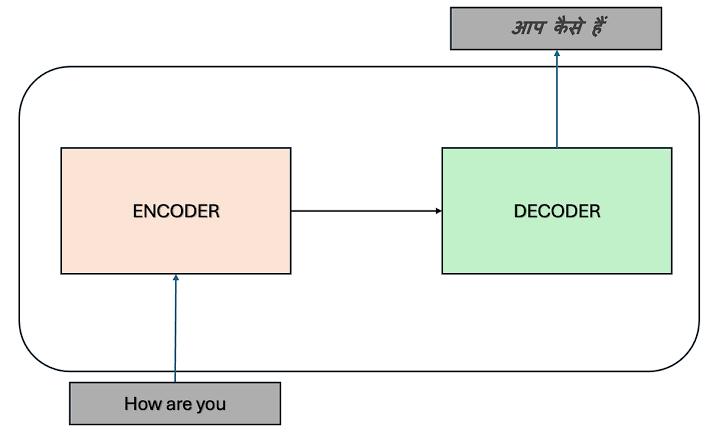
\includegraphics[width=0.6\textwidth]{../assets/figures/ch01-encoder-decoder.png}}
\caption{معماری \eng{Encoder-Decoder} در ترجمه: جملهٔ انگلیسی \eng{How are you} وارد رمزگذار می‌شود و رمزگشا معادل هندی آن را تولید می‌کند. \textit{(برگرفته از تختهٔ کلاس)}}
\label{fig:ch01-encdec}
\end{figure}

\subsection{طبقه‌بندی (\eng{Classification})}
در طبقه‌بندی، خروجی یکی از کلاس‌های از پیش‌تعریف‌شده است. استاد وظایف طبقه‌بندی را به دو گروه «تک‌جمله‌ای» و «دوجمله‌ای» تقسیم کرد.

\subsubsection{تحلیل احساسات (\eng{Sentiment Analysis})}
وظیفهٔ تک‌جمله‌ای: مدل احساس یا جهت‌گیری متن را تشخیص می‌دهد. تعداد کلاس‌ها به تعریف مسئله بستگی دارد؛ مثلاً سه‌کلاسه (مثبت، منفی، خنثی) یا پنج‌کلاسه: \eng{Strong Negative}، \eng{Negative}، \eng{Neutral}، \eng{Positive}، \eng{Strong Positive}.

\subsubsection{استنتاج زبان طبیعی (\eng{NLI})}
\eng{Natural Language Inference} وظیفه‌ای دوجمله‌ای است. استاد تأکید کرد که نام وظایف در \eng{NLP} معنای قراردادی دارد و صرفاً فهمیدن معنای لغوی نام برای شناخت دقیق وظیفه کافی نیست. در \eng{NLI} دو متن به مدل داده می‌شود: \term{مقدمه}{Premise} و \term{فرضیه}{Hypothesis}. مدل باید رابطهٔ آن‌ها را در یکی از سه کلاس قرار دهد:

\begin{table}[htbp]
\centering
\caption{سه کلاس \eng{NLI}}
\begin{tabular}{p{3.5cm}p{9.5cm}}
\toprule
کلاس & مفهوم \\
\midrule
\eng{Entailment} (استلزام) & فرضیه از مقدمه قابل نتیجه‌گیری است. \\
\eng{Contradiction} (تناقض) & فرضیه با مقدمه تناقض دارد. \\
\eng{Neutral} (خنثی) & از مقدمه نمی‌توان درستی یا نادرستی فرضیه را نتیجه گرفت. \\
\bottomrule
\end{tabular}
\end{table}

\paragraph{مثال کلاس.} مقدمه: «سامانهٔ راداری یک پهپاد ناشناس را شناسایی کرده است؛ به واحد پدافند ابلاغ شده که تا زمان شناسایی قطعی توسط گشت، از شلیک خودداری کند.»
\begin{itemize}
  \item الف) «واحد پدافند در حال حاضر دستور عدم درگیری را اجرا می‌کند.» برچسب موردنظر در کلاس: \eng{Entailment}
  \item ب) «واحد پدافند دستور دارد بلافاصله هر شیء متحرک در آسمان را با آتش سنگین منهدم کند.» برچسب: \eng{Contradiction}
  \item ج) «پهپاد حامل محموله غیرمجاز است.» برچسب: \eng{Neutral}، زیرا مقدمه دربارهٔ نوع محموله اطلاعاتی نمی‌دهد.
\end{itemize}

\begin{correctionbox}{برچسب فرضیهٔ «الف» وابسته به دستورالعمل برچسب‌گذاری است}
از نظر استنتاج منطقی سخت‌گیرانه، «دستور خودداری از شلیک داشتن» لزوماً به معنای «در حال حاضر در حال اجرای دستور عدم درگیری بودن» نیست؛ این فرضیه در بسیاری از دستورالعمل‌ها می‌تواند \eng{Neutral} یا استلزامِ ضعیف (به‌معنای «محتملاً درست») تلقی شود. در مجموعه‌داده‌های \eng{NLI} معمولاً از برچسب‌گذار خواسته می‌شود فرض کند مقدمه درست است و بپرسد «آیا یک انسان معقول فرضیه را نتیجه می‌گیرد؟». برچسب بالا مطابق بیان استاد حفظ شده و نشان می‌دهد چرا تعریف دقیق دستورالعمل مهم است.
\end{correctionbox}

\paragraph{اهمیت درک معنایی.} در مجموعه‌داده‌های ساده و قدیمی‌تر، گاهی رابطهٔ دو جمله با شباهت‌های واژگانی ساده قابل تشخیص بود. در مسائل پیچیده‌تر مدل باید بازنویسی‌های مختلف یک مفهوم را بفهمد؛ مثلاً «خودداری از شلیک» و «عدم درگیری» در یک بافت مشخص مفهوم نزدیکی دارند. در کاربردهای تخصصی نمی‌توان فرض کرد همهٔ مدل‌های عمومی چنین روابطی را درست تشخیص می‌دهند.

\subsubsection{شباهت معنایی متون (\eng{STS})}
\eng{Semantic Textual Similarity} نیز دوجمله‌ای است: ورودی دو جمله یا قطعه متن و خروجی یک امتیاز شباهت است. هدف بررسی یکسان بودن کلمات نیست، بلکه سنجش نزدیکی \emph{معنایی} دو متن است. در مثال کلاس، امتیاز در بازهٔ ۱ تا ۵ تعریف شد (نزدیک ۱: شباهت کم؛ نزدیک ۵: شباهت زیاد). اگر خروجی فقط مقادیر گسستهٔ ۱ تا ۵ باشد و هر عدد یک کلاس تلقی شود، مسئله \term{طبقه‌بندی}{Classification} است؛ اگر خروجی مقادیر پیوسته مانند $2.5$ یا $3.7$ بگیرد، مسئله \term{رگرسیون}{Regression} است. بنابراین نوع مسئله به نحوهٔ تعریف برچسب‌های مجموعه‌داده بستگی دارد.

\begin{correctionbox}{بازهٔ نمرهٔ \eng{STS}}
بازهٔ ۱ تا ۵ مثال کلاس است. در مجموعه‌داده‌های معروف \eng{STS} (مثل \eng{STS Benchmark}) نمره معمولاً پیوسته و در بازهٔ ۰ تا ۵ است و بیشتر به‌صورت رگرسیون مدل می‌شود.
\end{correctionbox}

\subsection{ارزیابی طبقه‌بندی: ماتریس درهم‌ریختگی و معیارها}
\subsubsection{چهار حالت پایه}
در طبقه‌بندی دودویی هر پیش‌بینی در یکی از چهار حالت زیر قرار می‌گیرد (شکل~\ref{fig:ch01-confusion}):
\begin{itemize}
  \item \term{مثبت درست}{True Positive, TP}: نمونهٔ مثبت را مثبت تشخیص داده‌ایم.
  \item \term{منفی درست}{True Negative, TN}: نمونهٔ منفی را منفی تشخیص داده‌ایم.
  \item \term{مثبت کاذب}{False Positive, FP}: نمونهٔ منفی را به‌اشتباه مثبت تشخیص داده‌ایم.
  \item \term{منفی کاذب}{False Negative, FN}: نمونهٔ مثبت را به‌اشتباه منفی تشخیص داده‌ایم.
\end{itemize}

\boardfigure{0.45}{ch01-confusion-matrix.png}{ماتریس درهم‌ریختگی (ردیف‌ها: برچسب واقعی، ستون‌ها: پیش‌بینی) و فرمول‌های دقت (\eng{Precision}) و بازیابی (\eng{Recall}).\label{fig:ch01-confusion}}

در مثال کلاس برای سادگی، کلاس \eng{Neutral} حالت «منفی» و دو کلاس \eng{Entailment} و \eng{Contradiction} حالت «مثبت» گرفته شدند. در مسائل چندکلاسه، تعریف مثبت و منفی به نحوهٔ ارزیابی بستگی دارد و هر کلاس را می‌توان جداگانه در برابر بقیه سنجید.

\subsubsection{دقت، بازیابی و \eng{F1}}
\begin{definitionbox}{معیارهای ارزیابی}
\[
\text{\lr{Precision}}=\frac{TP}{TP+FP},\qquad
\text{\lr{Recall}}=\frac{TP}{TP+FN},\qquad
F_1=2\cdot\frac{\text{\lr{Precision}}\cdot\text{\lr{Recall}}}{\text{\lr{Precision}}+\text{\lr{Recall}}}
\]
\eng{Precision}: از میان آنچه مثبت پیش‌بینی کرده‌ایم، چه کسری واقعاً مثبت است. \eng{Recall}: از میان نمونه‌های واقعاً مثبت، چه کسری را پیدا کرده‌ایم. \eng{F1} میانگین هارمونیک این دو است.
\end{definitionbox}

\begin{addedbox}{مثال عددی: محاسبهٔ دقت، بازیابی و \eng{F1}}
فرض کنید یک آشکارساز کلمهٔ فعال‌ساز روی ۱۰۰۰ قطعهٔ صوتی آزمایش شده است. ۶۰ قطعه واقعاً حاوی کلمهٔ فعال‌ساز بوده‌اند. ماتریس درهم‌ریختگی چنین است:
\begin{center}
\begin{tabular}{c|cc}
\toprule
 & پیش‌بینی: مثبت & پیش‌بینی: منفی \\
\midrule
واقعی: مثبت & $TP=40$ & $FN=20$ \\
واقعی: منفی & $FP=10$ & $TN=930$ \\
\bottomrule
\end{tabular}
\end{center}
\[
\text{\lr{Precision}}=\frac{40}{40+10}=0.80,\qquad
\text{\lr{Recall}}=\frac{40}{40+20}\approx0.667,
\]
\[
F_1=2\cdot\frac{0.80\times0.667}{0.80+0.667}\approx0.727
\quad\Bigl(\text{یا}\ \ F_1=\tfrac{2TP}{2TP+FP+FN}=\tfrac{80}{110}\Bigr).
\]
دقتِ کلی (\eng{Accuracy}) برابر $\frac{40+930}{1000}=0.97$ است، یعنی عددی بسیار بالا، در حالی که یک‌سوم کلمات فعال‌ساز تشخیص داده نشده‌اند. این نشان می‌دهد چرا در داده‌های نامتوازن \eng{Accuracy} به‌تنهایی گمراه‌کننده است و چرا \eng{Precision}، \eng{Recall} و \eng{F1} لازم‌اند.
\end{addedbox}

\subsubsection{هزینهٔ خطا در کاربردهای مختلف}
استاد دو مثال برای اهمیت نوع خطا مطرح کرد:
\begin{itemize}
  \item \textbf{سامانهٔ دفاعی}: مثبت کاذب (مثلاً تشخیص اشتباه یک شیء بی‌خطر به‌عنوان تهدید) می‌تواند به اقدام خطرناک منجر شود؛ پس نسبت به \eng{FP} حساسیت ویژه لازم است (دقت اهمیت بالایی دارد).
  \item \textbf{غربالگری بیماری}: از دست دادن یک فرد بیمار (منفی کاذب) می‌تواند پیامد جدی داشته باشد؛ پس کاهش \eng{FN} و افزایش \eng{Recall} مهم است.
\end{itemize}

\begin{exambox}{نتیجهٔ مهم}
معیار ارزیابی را نباید صرفاً با یک عدد عمومی انتخاب کرد؛ باید با نیازمندی و حساسیت کاربرد هماهنگ باشد. معمولاً بالا بردن دقت و بازیابی هم‌زمان دشوار است و میان آن‌ها مصالحه (\eng{trade-off}) وجود دارد.
\end{exambox}

\subsection{برچسب‌گذاری توالی (\eng{Sequence Labeling})}
در برچسب‌گذاری توالی، ورودی توالی‌ای از توکن‌هاست و برای هر توکن یک برچسب تولید می‌شود. روی تخته دو مجموعهٔ برچسب (\eng{tagset}) و یک جملهٔ نمونه نوشته شده است (شکل~\ref{fig:ch01-posner}).

\begin{figure}[htbp]
\centering
\resizebox{0.95\textwidth}{!}{%
\begin{tikzpicture}[rtl, font=\small,
  tagbox/.style={draw=mainblue, fill=softblue, rounded corners=4pt, align=center, inner sep=6pt},
  word/.style={font=\normalsize, inner sep=2pt},
  nertg/.style={draw=black!50, fill=softgreen, rounded corners=2pt, minimum width=1.5cm, minimum height=6mm, inner sep=2pt, font=\footnotesize},
  postg/.style={draw=black!50, fill=softred, rounded corners=2pt, minimum width=1.5cm, minimum height=6mm, inner sep=2pt, font=\footnotesize}]
\node[tagbox] at (3.6,5.2) {\lr{tagset POS}\\\lr{Noun, Proper Noun, Pronoun}\\\lr{Verb, Adverb, Adjective}\\\lr{Preposition, Adposition}};
\node[tagbox] at (11.2,5.2) {\lr{tagset NER}\\\lr{LOC, PER, ORG}};
\draw[rounded corners=5pt, draw=black!60] (-0.2,-1.9) rectangle (14.5,2.3);
\node[font=\footnotesize, anchor=west] at (0,1.9) {\lr{NER (IOB)}};
\node[font=\footnotesize, anchor=west] at (0,-1.5) {\lr{POS}};
\foreach \x/\w/\n/\p in {13/هواپیما/O/Noun, 11.2/شنبه/B-TIME/Noun, 9.4/از/O/Prep., 7.6/فرودگاه/B-LOC/Noun, 5.8/مهرآباد/I-LOC/{Proper Noun}, 4.0/پرواز/O/Noun, 2.2/کرد/O/Verb} {
  \node[word] (w\x) at (\x,0) {\w};
  \node[nertg] at (\x,1.2) {\lr{\n}};
  \node[postg] at (\x,-1.2) {\lr{\p}};
}
\end{tikzpicture}}
\caption{مجموعهٔ برچسب‌های \eng{POS} و \eng{NER} و برچسب‌گذاری جملهٔ نمونهٔ «هواپیما شنبه از فرودگاه مهرآباد پرواز کرد»: برچسب‌های \eng{NER} با قالب \eng{IOB} بالای جمله (سبز) و برچسب‌های \eng{POS} زیر آن (قرمز) آمده‌اند؛ کلمات از راست به چپ خوانده می‌شوند. روی تخته برچسب‌ها به‌صورت اختصاری (\eng{N}، \eng{V}، \eng{P}، \eng{B-LOC}، \eng{I-LOC}، \ldots) نوشته شده بود. (بازسازی‌شده از تختهٔ کلاس)}
\label{fig:ch01-posner}
\end{figure}

\subsubsection{برچسب‌گذاری نقش واژگانی (\eng{POS Tagging})}
برای هر کلمه، دستهٔ دستوری آن (\eng{Noun}، \eng{Proper Noun}، \eng{Pronoun}، \eng{Verb}، \eng{Adjective}، \eng{Adverb}، \eng{Preposition} یا \eng{Adposition}) مشخص می‌شود. استاد تأکید کرد \eng{POS Tagging} با تعیین نقش نحوی (فاعل، مفعول و ...) فرق دارد: یک اسم خاص در یک جمله فاعل و در جمله‌ای دیگر مفعول است، ولی دستهٔ واژگانی‌اش همچنان «اسم خاص» است.

\subsubsection{قالب \eng{IOB} و شناسایی موجودیت‌های نام‌دار (\eng{NER})}
وقتی چند کلمهٔ متوالی به یک موجودیت تعلق دارند، مرز عبارت با قالب \eng{IOB} مشخص می‌شود:
\begin{itemize}
  \item \eng{B} (\eng{Beginning}): شروع یک عبارت برچسب‌دار،
  \item \eng{I} (\eng{Inside}): ادامهٔ عبارت،
  \item \eng{O} (\eng{Outside}): خارج از هر عبارت موردنظر.
\end{itemize}
\term{شناسایی موجودیت نام‌دار}{Named Entity Recognition - NER} موجودیت‌های مهم متن را پیدا و دسته‌بندی می‌کند. دسته‌های رایج: شخص (\eng{PER})، مکان (\eng{LOC})، سازمان (\eng{ORG}) و زمان/تاریخ. تعداد و نوع دسته‌ها به مسئله بستگی دارد؛ مثلاً در یک پروژهٔ تخصصی ممکن است هدف شناسایی نام حیوانات یا گیاهان باشد. این انتخاب به مفاهیم و رده‌بندی‌ای که کارفرما نیاز دارد وابسته است و به مفهوم \term{هستی‌شناسی}{Ontology} مربوط می‌شود.

در کلاس دربارهٔ کلمهٔ «شنبه» و فعل مرکب «پرواز کرد» بحث شد. برچسب‌گذاری چنین مواردی باید طبق دستورالعمل مشخص مجموعه‌داده باشد؛ مثلاً ممکن است یک نظام برچسب‌گذاری برای اجزای فعل مرکب برچسب‌های جدا بگذارد. بنابراین برچسب‌های شکل~\ref{fig:ch01-posner} نمونه‌ای مطابق بحث کلاس‌اند و تنها برچسب‌گذاری معتبر نیستند.

\subsubsection{ارزیابی \eng{NER}}
می‌توان از \eng{Precision}، \eng{Recall} و \eng{F1} استفاده کرد. در بحث کلاس، \eng{O} حالت «منفی» در نظر گرفته شد: اگر کلمه‌ای در داده مرجع \eng{O} باشد ولی مدل آن را مکان تشخیص دهد، یک مثبت کاذب رخ داده است.

\begin{correctionbox}{ارزیابی در سطح توکن یا در سطح موجودیت}
در ارزیابی استاندارد \eng{NER} (مثل \eng{conlleval} و \eng{seqeval}) معمولاً یک موجودیت تنها وقتی درست شمرده می‌شود که \emph{هم نوع و هم مرز} آن کاملاً درست باشد (مثلاً «فرودگاه مهرآباد» باید با هر دو توکن و برچسب‌های \eng{B-LOC}، \eng{I-LOC} پیدا شود). اگر فقط توکن‌ها شمرده شوند، چون اکثر توکن‌ها \eng{O} هستند، دقت کلی بسیار بالا و گمراه‌کننده می‌شود؛ به همین دلیل \eng{F1} در سطح موجودیت گزارش می‌شود.
\end{correctionbox}

\subsubsection{دستورالعمل برچسب‌گذاری (\eng{Annotation Guideline})}
در پروژه‌های واقعی، مهندس هوش مصنوعی لزوماً مسئول همهٔ جزئیات زبان‌شناختی نیست و ممکن است برای طراحی دقیق برچسب‌ها از یک زبان‌شناس کمک بگیرد. مراحل کار:
\begin{enumerate}
  \item تعیین هدف پروژه و اطلاعات موردنیاز،
  \item تعریف مجموعهٔ برچسب‌ها (\eng{Tag Set})،
  \item تدوین دستورالعمل برچسب‌گذاری با کمک متخصص زبان،
  \item آموزش برچسب‌گذاران،
  \item برچسب‌گذاری داده‌ها بر اساس دستورالعمل مشترک،
  \item بررسی سازگاری و کیفیت برچسب‌ها.
\end{enumerate}
همین دستورالعمل می‌تواند مبنای \eng{Prompt} برای برچسب‌گذاری با مدل‌های زبانی هم باشد. بنابراین طراحی یک مجموعه‌داده فقط انتخاب مدل نیست؛ تعریف دقیق برچسب‌ها و قواعد استفاده از آن‌ها نیز اهمیت دارد.

\subsection{تشخیص قصد و پر کردن جایگاه‌ها (\eng{Intent Detection and Slot Filling})}
این دو وظیفه در سامانه‌های مکالمه‌ای و دستیارهای صوتی با هم به‌کار می‌روند:
\begin{itemize}
  \item \term{تشخیص قصد}{Intent Detection}: کل جمله در یک کلاس (مثل سفارش غذا، درخواست تاکسی، خرید، کنترل وسایل هوشمند) قرار می‌گیرد؛ پس طبقه‌بندی در سطح جمله است.
  \item \term{پر کردن جایگاه}{Slot Filling}: استخراج اطلاعات لازم برای اجرای قصد (مثلاً نوع غذا، نام رستوران، آدرس تحویل). \eng{Slot Filling} معمولاً به‌صورت برچسب‌گذاری توالی (با قالب \eng{IOB}) مدل می‌شود.
\end{itemize}

\begin{figure}[htbp]
\centering
\resizebox{\textwidth}{!}{%
\begin{tikzpicture}[rtl, font=\small,
  word/.style={font=\normalsize, inner sep=2pt},
  tg/.style={draw=black!50, fill=softred, rounded corners=2pt, minimum width=1.45cm, minimum height=6mm, inner sep=2pt, font=\footnotesize},
  slot/.style={draw=mainblue, fill=softblue, rounded corners=3pt, minimum height=7mm, inner sep=3pt, font=\footnotesize, align=center}]
\draw[rounded corners=5pt, draw=black!60] (-0.4,-0.8) rectangle (16.9,0.8);
\foreach \x/\w/\t in {16/دو/O, 14.5/تا/O, 13/چلوکباب/B-FOOD, 11.5/از/O, 10/تهیه/B-REST, 8.5/غذای/I-REST, 7/فارسی/I-REST, 5.5/به/O, 4/آدرس/B-ADDR, 2.5/خودم/I-ADDR} {
  \node[word] at (\x,0) {\w};
  \node[tg] at (\x,-1.6) {\lr{\t}};
}
% intent
\node[slot, fill=softyellow, draw=black!60] (int) at (9.35,3.9) {\lr{Intent: OrderFood}\\{\footnotesize (قصد: سفارش غذا)}};
\draw[decorate, decoration={brace, amplitude=6pt}, thick, mainblue] (2.0,1.0) -- (16.7,1.0);
\draw[-{Stealth}, thick, mainblue] (int.south) -- (9.35,1.7);
% slots
\node[slot] at (13,-2.7) {\lr{Slot: FOOD}\\{\footnotesize (غذا)}};
\node[slot] at (8.5,-2.7) {\lr{Slot: RESTAURANT}\\{\footnotesize (رستوران)}};
\node[slot] at (3.25,-2.7) {\lr{Slot: ADDRESS}\\{\footnotesize (آدرس)}};
\end{tikzpicture}}
\caption{جملهٔ نمونهٔ «دو تا چلوکباب از تهیه‌غذای فارسی به آدرس خودم» (خوانش از راست به چپ): کل جمله یک قصد (\eng{Intent}) دارد و هر توکن با قالب \eng{IOB} برچسب جایگاه (\eng{Slot}) می‌گیرد. روی تخته جایگاه‌ها با حرف اختصاری (\eng{N} برای غذا، \eng{R} برای رستوران و \eng{A} برای آدرس) نوشته شده بودند. (بازسازی‌شده از تختهٔ کلاس)}
\label{fig:ch01-intent-slot}
\end{figure}

\paragraph{مثال کلاس.} جملهٔ «دو تا چلوکباب از تهیه‌غذای فارسی به آدرس خودم» با قصد \eng{OrderFood} در شکل~\ref{fig:ch01-intent-slot} برچسب‌گذاری شده است: «چلوکباب» نام غذا (\eng{B-FOOD})، «تهیه‌غذای فارسی» نام رستوران (\eng{B-REST} و دو \eng{I-REST}) و «آدرس خودم» آدرس تحویل (\eng{B-ADDR}، \eng{I-ADDR}) است و بقیهٔ توکن‌ها \eng{O} هستند.
در این مثال فرض شده مجموعهٔ جایگاه‌ها فقط نام غذا، رستوران و آدرس است، پس «دو تا» برچسب \eng{O} گرفته است؛ اگر تعداد غذا هم مهم باشد، می‌توان جایگاه جداگانه‌ای مثل \eng{Quantity} تعریف کرد. یعنی برچسب‌گذاری به طرح داده (\eng{Data Schema}) و نیازمندی‌ها وابسته است.

\begin{definitionbox}{قصد و جایگاه}
\textbf{قصد} (\eng{Intent}): هدف کاربر از جمله. \textbf{جایگاه} (\eng{Slot}): پارامترهای لازم برای اجرای آن هدف. مثلاً قصد «خرید بلیت» جایگاه‌های مبدأ، مقصد و ساعت دارد.
\end{definitionbox}

\paragraph{پرسش و پاسخ: اگر کاربر قصدش را مستقیم نگوید؟} مثلاً به‌جای «کولر را روشن کن» بگوید «هوا خیلی گرم است». اینکه مدل این جمله را قصد روشن کردن کولر بداند به داده‌های آموزشی و تعریف مسئله بستگی دارد: اگر در داده‌ها شکایت از گرما در آن بافت به‌معنای درخواست روشن کردن کولر باشد، مدل می‌تواند آن را یاد بگیرد؛ در این حالت قصد به کل جمله نسبت داده می‌شود، نه فقط کلمهٔ «گرم». اگر جمله جایگاه‌های لازم را نداشته باشد، سیستم می‌تواند وارد گفت‌وگو شود و اطلاعات ناقص را بپرسد:

\begin{quote}
کاربر: «می‌خوام غذا سفارش بدم.» \quad سیستم: «چه غذایی می‌خواهید؟ از کدام رستوران؟»
\end{quote}

\subsection{مدل‌سازی زبان و سه الگوی معماری}
\subsubsection{مدل‌سازی زبان علّی}
در مدل‌سازی زبان (\eng{Language Modeling - Causal LM}) مدل توالی‌ای از توکن‌ها را می‌گیرد و توکن بعدی را پیش‌بینی می‌کند؛ با تکرار این کار متن کامل تولید می‌شود:
\[
P(x_t\mid x_1,x_2,\ldots,x_{t-1}).
\]
به این شیوه «علّی» (\eng{Causal}) گفته می‌شود، چون مدل هنگام پیش‌بینی فقط به توکن‌های قبلی تکیه می‌کند.

\subsubsection{انواع معماری \eng{Transformer}}
\begin{itemize}
  \item \textbf{\eng{Encoder-only}}: برای درک و استخراج بازنمایی از ورودی؛ مناسب وظایف طبقه‌بندی مانند تحلیل احساسات و برچسب‌گذاری.
  \item \textbf{\eng{Decoder-only}}: تولید خودبازگشتی (\eng{autoregressive}) توکن‌ها؛ مناسب مدل‌سازی زبان و تولید متن (مانند خانوادهٔ \eng{GPT}).
  \item \textbf{\eng{Encoder-Decoder}}: بازنمایی ورودی و تولید خروجی جدید؛ مناسب وظایف \eng{Seq2Seq} مانند ترجمه و خلاصه‌سازی.
\end{itemize}

\paragraph{پرسش و پاسخ: آیا \eng{Decoder-only} یعنی مدل ورودی را نمی‌فهمد؟} خیر. \eng{Decoder-only} یعنی معماری یک \eng{Encoder} مجزا مانند \eng{Encoder-Decoder} ندارد؛ ولی مدل با لایه‌های خود ورودی و زمینهٔ آن را پردازش می‌کند و بر اساس آن خروجی می‌سازد. \eng{Prompt} همان ورودی متنی مدل است که در پردازش و تولید پاسخ نقش دارد. جزئیات \eng{Transformer} در جلسات بعد بررسی می‌شود.

\begin{correctionbox}{نکتهٔ تکمیلی دربارهٔ معماری‌ها}
تقسیم‌بندی بالا نمای کلی و ساده‌شده است. مدل‌های \eng{Encoder-only} (مانند \eng{BERT}) معمولاً با هدف «مدل‌سازی زبان پوشیده» (\eng{Masked LM}) آموزش می‌بینند، نه پیش‌بینی توکن بعدی؛ و مدل‌های \eng{Decoder-only} امروزه با \eng{Prompt} طبقه‌بندی و برچسب‌گذاری را هم انجام می‌دهند. پس این وظایف را «مناسب» هر معماری می‌دانیم، نه «منحصر» به آن.
\end{correctionbox}

\subsection{هم‌ارجاعی، پیوند موجودیت و خوشه‌بندی}
\subsubsection{تشخیص هم‌ارجاعی (\eng{Coreference Resolution})}
باید عبارت‌هایی که به یک موجودیت مشترک اشاره دارند شناسایی شوند. ورودی یک متن یا سند و خروجی گروه‌هایی از عبارت‌های هم‌ارجاع است. مثلاً اگر ابتدا نام «علی» بیاید و بعد «آقای احمدی» یا «او»، مدل باید بفهمد همه به یک شخص اشاره می‌کنند:
\begin{itemize}
  \item \textbf{خوشهٔ ۱}: علی، آقای احمدی، او
  \item \textbf{خوشهٔ ۲}: کتاب، این اثر، آن
\end{itemize}
از نظر ساختار خروجی، این مسئله به \term{خوشه‌بندی}{Clustering} شباهت دارد، چون تعداد خوشه‌ها و اعضای هر خوشه از پیش معلوم نیست (در تخته: «خوشه‌بندی عبارات اسمی و ضمایر که هویت ارجاعی یکسانی در متن دارند»).

\subsubsection{پیوند موجودیت (\eng{Entity Linking})}
در کلاس تفاوت چنین بیان شد: هم‌ارجاعی درون یک سند و \eng{Entity Linking} ایجاد ارتباط میان اشاره‌ها در اسناد مختلف.

\begin{correctionbox}{تعریف دقیق \eng{Entity Linking}}
بیان کلاس ساده‌سازی است. در تعریف رایج، \term{پیوند موجودیت}{Entity Linking} یعنی نگاشت هر \emph{اشاره} (\eng{mention}) در متن به یک موجودیت مشخص در یک پایگاه دانش (مثل ویکی‌پدیا یا \eng{Wikidata}). مثلاً «مهرآباد» در یک متن به مدخل «فرودگاه بین‌المللی مهرآباد» وصل می‌شود، نه به مکانی هم‌نام. هم‌ارجاعی میان‌اسنادی (\eng{Cross-document Coreference}) مسئلهٔ نزدیک ولی جداست.
\end{correctionbox}

\section{وظایف پردازش گفتار}
تأکید اصلی درس بر وظایف گفتاری و مدل‌های آن‌ها خواهد بود. فهرست این وظایف روی تخته در شکل~\ref{fig:ch01-speech-board} آمده است.

\begin{figure}[htbp]
\centering
\resizebox{\textwidth}{!}{%
\begin{tikzpicture}[rtl, font=\small, >=Stealth,
  task/.style={draw=mainblue, fill=softblue, rounded corners=3pt, minimum height=8mm, minimum width=6.4cm, align=center, inner sep=4pt},
  note/.style={draw=black!50, fill=softyellow, rounded corners=3pt, align=center, inner sep=5pt, text width=5.4cm, font=\footnotesize},
  grn/.style={draw=black!40, fill=softgreen, rounded corners=3pt, align=center, inner sep=5pt, font=\footnotesize}]
\node[task] (asr) at (0,0) {\lr{Streaming STT/ASR}\\{\footnotesize \lr{(Automatic Speech Recognition)}}};
\node[task] (tts) at (0,-1.3) {\lr{Streaming TTS}};
\node[task] (ns) at (0,-2.4) {\lr{Noise Suppression}};
\node[task] (vad) at (0,-3.5) {\lr{VAD}\\{\footnotesize \lr{(Voice Activity Detection)}}};
\node[task] (ww) at (0,-4.8) {\lr{Wake Word}};
\node[task] (s2i) at (0,-5.9) {\lr{Speech-to-Intent}};
\node[task] (sr) at (0,-7.0) {\lr{Speaker Recognition}};
\node[task] (sd) at (0,-8.1) {\lr{Speaker Diarization}};
\node[grn] (mode) at (-5.9,-0.3) {\lr{Batch / Non-streaming}\\\lr{Real time}\\\lr{Latency}};
\draw[->, thick, black!60] (mode.east) -- (asr.west);
\node[note] (wwn) at (6.6,-4.8) {تا زمانی که کلمهٔ بیدارباش شنیده نشود، مدل‌های سنگین‌تر، یعنی \lr{ASR}، \lr{Intent Detection} و \lr{LLM}ها، اصلاً روشن نمی‌شوند.};
\draw[->, thick, black!60] (wwn.west) -- (ww.east);
\end{tikzpicture}}
\caption{فهرست وظایف گفتاری روی تخته. کادر سبز: تفاوت حالت دسته‌ای (\eng{Batch/Non-streaming}) و بلادرنگ (\eng{Real-time}) و اهمیت تأخیر (\eng{Latency}) در بازشناسی گفتار؛ کادر زرد: یادداشت استاد دربارهٔ روشن نشدن مدل‌های سنگین پیش از شنیدن کلمهٔ بیدارباش. (بازسازی‌شده از تختهٔ کلاس)}
\label{fig:ch01-speech-board}
\end{figure}

\subsection{بازشناسی خودکار گفتار (\eng{ASR})}
\term{بازشناسی خودکار گفتار}{Automatic Speech Recognition - ASR}، یا \eng{Speech-to-Text (STT)}، گفتار را به متن تبدیل می‌کند: ورودی سیگنال صوتی و خروجی متن. مثلاً «چراغ اتاق را خاموش کن.»

\subsubsection{حالت غیرجریانی و جریانی}
\begin{itemize}
  \item \term{غیرجریانی (دسته‌ای)}{Non-streaming / Batch}: ابتدا بخش کامل گفتار (مثلاً یک فایل ضبط‌شده) دریافت و سپس پردازش می‌شود. چون مدل به کل گفتار دسترسی دارد، معمولاً زمینهٔ بیشتری برای تشخیص دارد.
  \item \term{جریانی}{Streaming / Real-time}: سیستم هم‌زمان با دریافت گفتار شروع به پردازش می‌کند و منتظر پایان جمله نمی‌ماند. در دستیارهای صوتی و کاربردهای بلادرنگ مهم است.
\end{itemize}

\begin{table}[htbp]
\centering
\caption{مقایسهٔ حالت جریانی و غیرجریانی}
\begin{tabular}{p{3.5cm}p{4.8cm}p{4.8cm}}
\toprule
ویژگی & جریانی & غیرجریانی \\
\midrule
شروع پردازش & هنگام دریافت صوت & پس از دریافت بخش کامل \\
تأخیر پاسخ & معمولاً کمتر & معمولاً بیشتر \\
زمینهٔ در دسترس & محدودتر & بیشتر \\
پیچیدگی طراحی & بیشتر & معمولاً کمتر \\
کاربرد & تعامل زنده & پردازش فایل‌های ضبط‌شده \\
\bottomrule
\end{tabular}
\end{table}

در شرایط مشابه، پردازش غیرجریانی با استفاده از زمینهٔ کامل معمولاً به دقت بهتری می‌رسد، در حالی که حالت جریانی برای کاهش تأخیر طراحی می‌شود. روی تخته سه واژهٔ «\eng{Batch / Non-streaming}»، «\eng{real time}» و «\eng{Latency}» کنار هم نوشته شده است.

\subsubsection{قطعه‌بندی (\eng{Chunking}) در داده‌های جریانی}
در حالت غیرجریانی ممکن است کل جمله یک نمونهٔ ورودی باشد؛ اما مدل جریانی باید سیگنال را به قطعات کوچک به نام \term{چانک}{Chunk} تقسیم کند. فرض کنید می‌خواهیم قصد کاربر را هنگام دریافت جملهٔ «چراغ اتاق را خاموش کن» تشخیص دهیم. در هر مرحله فقط بخشی از جمله در دسترس است: چانک ۱: «چراغ»؛ چانک ۲: «چراغ اتاق را»؛ چانک ۳: «چراغ اتاق را خاموش کن». برای ساخت داده می‌توان قطعاتی از گفتار ساخت و در یک طراحی مشخص برچسب \eng{Intent} جملهٔ کامل را به آن‌ها هم داد. البته در مراحل اولیه مدل اطلاعات کافی ندارد: با شنیدن «چراغ اتاق را...» هنوز معلوم نیست قصد روشن کردن است یا خاموش کردن. استاد به \term{هم‌پوشانی}{Overlap} میان قطعات هم اشاره کرد: بخشی از صوت در چند چانک متوالی تکرار می‌شود تا پیوستگی اطلاعات حفظ شود؛ این کار می‌تواند مؤثر باشد ولی باید با طراحی مناسب داده و مدل همراه باشد.

\begin{figure}[htbp]
\centering
\begin{tikzpicture}[font=\small, x=2.2cm,
  ch/.style={draw, rounded corners=2pt, minimum height=6mm, fill=softblue}]
\draw[thick, -{Stealth}] (0,0) -- (4.3,0) node[below left] {\lr{time (s)}};
\foreach \t in {0,1,2,3,4} \draw (\t,0.07)--(\t,-0.07) node[below] {\lr{\t}};
\foreach \i/\s/\n in {0/0/1, 1/0.5/2, 2/1/3, 3/1.5/4} {
  \node[ch, anchor=south west, minimum width=2.2cm] at (\s,0.25+\i*0.75) {\lr{chunk \n}};
}
\end{tikzpicture}
\caption{چانک‌های یک‌ثانیه‌ای با گام نیم‌ثانیه‌ای؛ هر چانک ۵۰\% با چانک قبلی هم‌پوشانی دارد (شکل افزوده).}
\end{figure}

\begin{addedbox}{مثال عددی: تعداد چانک‌ها}
فرض کنید طول چانک $L=1$ ثانیه، گام (\eng{hop}) برابر $H=0.5$ ثانیه (هم‌پوشانی ۵۰\%) و طول گفتار $T=4$ ثانیه باشد. تعداد چانک‌های کامل
\[
N=\Bigl\lfloor\frac{T-L}{H}\Bigr\rfloor+1=\Bigl\lfloor\frac{4-1}{0.5}\Bigr\rfloor+1=7.
\]
بدون هم‌پوشانی ($H=L$) فقط ۴ چانک داریم. مدل جریانی ناچار است دست‌کم یک چانک (در اینجا ۱ ثانیه) صبر کند، پس تأخیرِ حداقلی سیستم به طول چانک وابسته است؛ چانک کوچک‌تر تأخیر را کم، ولی زمینه و معمولاً دقت را کمتر می‌کند.
\end{addedbox}

\subsection{تبدیل متن به گفتار (\eng{TTS})}
\term{تبدیل متن به گفتار}{Text-to-Speech - TTS} معکوس \eng{ASR} است: ورودی متن (مثلاً «سلام، حال شما چطور است؟») و خروجی سیگنال گفتار. در \term{\eng{TTS} جریانی}{Streaming TTS} تولید گفتار تدریجی انجام می‌شود و سیستم پیش از آماده شدن کل پاسخ می‌تواند صوت را پخش کند؛ این برای سامانه‌های مکالمه‌ای بلادرنگ مهم است.

\subsection{حذف نویز (\eng{Noise Suppression})}
ورودی صوت نویزی و خروجی نسخهٔ بهبودیافتهٔ آن است. در مدل ساده‌ای که در کلاس بحث شد، گفتار اصلی حفظ و نویز کم می‌شود و \emph{طول فایل تغییر نمی‌کند}: گفتار ۱۰ ثانیه‌ای با نویز محیط، به سیگنال ۱۰ ثانیه‌ای با نویز کمتر تبدیل می‌شود. این وظیفه (که به‌طور کلی \eng{Speech Enhancement} نام دارد) معمولاً از مراحل اولیهٔ خط لولهٔ پردازش گفتار است.

\subsection{تشخیص فعالیت گفتاری (\eng{VAD})}
\term{تشخیص فعالیت گفتاری}{Voice Activity Detection - VAD} مشخص می‌کند در کدام بازه‌های سیگنال گفتار وجود دارد. در ساده‌ترین شکل یک طبقه‌بندی دودویی است: \eng{0} یعنی گفتار نیست و \eng{1} یعنی گفتار هست. مثلاً اگر در پنج ثانیهٔ اول کسی صحبت نکند و بعد کاربر شروع کند، \eng{VAD} باید این تغییر وضعیت را تشخیص دهد.

\paragraph{کاربرد: صرفه‌جویی در منابع.} دستیار صوتی دائماً صدای محیط را دریافت می‌کند، ولی لازم نیست مدل‌های سنگین همیشه فعال باشند. می‌توان ابتدا \eng{VAD} را اجرا کرد و فقط با تشخیص فعالیت گفتاری مراحل بعدی را فعال کرد:
\[
\text{\lr{Audio}}\rightarrow\text{\lr{Noise Suppression}}\rightarrow\text{\lr{VAD}}\rightarrow\text{\lr{Speech Processing}}.
\]

\subsection{تشخیص کلمهٔ فعال‌ساز (\eng{Wake Word Detection})}
وظیفهٔ شناسایی یک کلمه یا عبارت مشخص برای فعال‌سازی سیستم است؛ کاربر از قبل می‌داند باید آن عبارت را بگوید (مثلاً «سلام»). سیستم ابتدا آن را تشخیص می‌دهد و بعد پردازش اصلی را آغاز می‌کند. روی تخته یادداشت شده: تا زمانی که کلمهٔ بیداری‌باش شنیده نشود، مدل‌های سنگین‌تر (\eng{ASR}، \eng{Intent Detection} و \eng{LLM}ها) اصلاً روشن نمی‌شوند.

\begin{table}[htbp]
\centering
\caption{تفاوت \eng{VAD} و \eng{Wake Word}}
\begin{tabular}{p{6.2cm}p{6.2cm}}
\toprule
\eng{VAD} & \eng{Wake Word Detection} \\
\midrule
وجود گفتار را تشخیص می‌دهد. & وجود یک عبارت مشخص را تشخیص می‌دهد. \\
به محتوای دقیق جمله وابسته نیست. & به کلمه یا عبارت هدف وابسته است. \\
برای شناسایی بازه‌های گفتاری به‌کار می‌رود. & برای فعال‌سازی دستیار به‌کار می‌رود. \\
\bottomrule
\end{tabular}
\end{table}

هر دو می‌توانند از اجرای دائمی مدل‌های پرهزینه جلوگیری کنند.

\subsection{تشخیص مستقیم قصد از گفتار (\eng{Speech-to-Intent})}
ورودی گفتار و خروجی برچسب قصد است و لزومی ندارد تبدیل صوت به متن در یک مرحلهٔ مستقل انجام شود. دو رویکرد قابل مقایسه‌اند:
\begin{gather*}
\text{\lr{Speech}}\rightarrow\text{\lr{ASR}}\rightarrow\text{\lr{Text}}\rightarrow\text{\lr{Intent Detection}}\\
\text{در برابر}\\
\text{\lr{Speech}}\rightarrow\text{\lr{Speech-to-Intent}}\rightarrow\text{\lr{Intent}}.
\end{gather*}
این ماژول می‌تواند در بخش‌های ابتدایی سیستم، به‌عنوان تصمیم‌گیرندهٔ سبک به‌کار رود: اگر کاربر فقط بگوید «چراغ را خاموش کن»، لازم نیست مدل زبانی بزرگ فعال شود و فرمان مستقیماً اجرا می‌شود. این رویکرد برای \eng{Edge AI} و کاربردهایی که مصرف منابع مهم است مفید است.

\subsection{بازشناسی گوینده (\eng{Speaker Recognition})}
هدف شناسایی گوینده از روی ویژگی‌های صدای اوست. مثال استاد: دستیار صوتی که فقط باید به دستور افراد مشخصی پاسخ دهد، در حالی که ممکن است رادیو روشن باشد یا شخص دیگری حرف بزند. روند:
\begin{enumerate}
  \item نمونهٔ صدای کاربران مجاز ثبت می‌شود.
  \item سیستم صدای جدیدی دریافت می‌کند.
  \item مدل ویژگی‌های گوینده را بررسی می‌کند.
  \item در صورت تطابق با کاربر مجاز، پردازش اصلی ادامه می‌یابد.
\end{enumerate}
بدین ترتیب این وظیفه می‌تواند جزئی از کنترل دسترسی یا شخصی‌سازی دستیار باشد.

\begin{correctionbox}{تشخیص هویت و تأیید هویت}
بازشناسی گوینده معمولاً دو حالت دارد: \term{تأیید گوینده}{Speaker Verification} (آیا این صدا مال همان کسی است که ادعا می‌کند؟ تصمیم دودویی) و \term{شناسایی گوینده}{Speaker Identification} (این صدا مال کدام‌یک از افراد ثبت‌شده است؟). مثال دستیار صوتی بالا بیشتر به تأیید نزدیک است.
\end{correctionbox}

\subsection{تفکیک گویندگان (\eng{Speaker Diarization})}
\term{تفکیک گویندگان}{Speaker Diarization} مشخص می‌کند \emph{چه کسی در چه زمانی} صحبت کرده است. خروجی یک \eng{ASR} معمولی برای یک جلسه فقط می‌تواند متن «سلام، جلسه شروع شد. مدارک کجاست؟ فرستادم خدمتتون.» باشد؛ ولی در \eng{Diarization} گفتار افراد جدا می‌شود و بازه‌های زمانی هم مشخص می‌گردد:

\begin{table}[htbp]
\centering
\caption{نمونهٔ خروجی \eng{Diarization} همراه با \eng{ASR} (مثال کلاس)}
\begin{tabular}{llp{6cm}}
\toprule
گوینده & زمان & متن \\
\midrule
گوینده ۱ (علی) & \eng{00:01} & سلام، جلسه شروع شد. \\
گوینده ۲ (رضا) & \eng{00:03} & مدارک کجاست؟ \\
گوینده ۱ (علی) & \eng{00:05} & فرستادم خدمتتون. \\
\bottomrule
\end{tabular}
\end{table}

استاد این وظیفه را از جهتی شبیه \eng{Coreference Resolution} دانست: همان‌طور که عبارت‌های دارای مرجع مشترک در یک خوشه قرار می‌گیرند، در \eng{Diarization} هم بخش‌های صوتیِ متعلق به یک گوینده در یک گروه قرار می‌گیرند؛ پس می‌توان آن را از نظر گروه‌بندی قطعات گفتار، مسئلهٔ \eng{Clustering} نیز دانست.

\begin{table}[htbp]
\centering
\caption{تفاوت بازشناسی گوینده و تفکیک گویندگان}
\begin{tabular}{p{3.2cm}p{4.9cm}p{4.9cm}}
\toprule
ویژگی & \eng{Speaker Recognition} & \eng{Speaker Diarization} \\
\midrule
پرسش اصلی & این صدا متعلق به چه کسی است؟ & چه کسی در چه زمانی صحبت کرده است؟ \\
نیاز به کاربران از پیش شناخته‌شده & در کاربرد کلاس، بله & الزاماً خیر \\
خروجی & هویت یا نتیجهٔ تطابق & بازه‌های زمانی تفکیک‌شده بر اساس گوینده \\
کاربرد & کنترل دسترسی صوتی & تحلیل جلسات و مکالمات چندنفره \\
\bottomrule
\end{tabular}
\end{table}

\section{وظایف بینایی و ارتباط آن‌ها با درس}
تمرکز اصلی درس بر مدل‌ها و وظایف گفتار است، اما در طراحی محصولات واقعی ممکن است به مدل‌های متن و تصویر هم نیاز باشد. دو مفهوم بینایی در کلاس معرفی شد:
\begin{itemize}
  \item \term{مدل‌های بینایی-زبان}{Vision-Language Models - VLM}: اطلاعات تصویری و متنی را با هم پردازش می‌کنند؛ مثلاً تصویری را می‌گیرند و به پرسش‌هایی دربارهٔ آن پاسخ می‌دهند. در برخی معماری‌ها ویدئو هم در کنار تصویر و متن پردازش می‌شود.
  \item \term{بازشناسی نوری نویسه}{Optical Character Recognition - OCR}: استخراج متن از تصویر؛ ورودی تصویر حاوی متن و خروجی متن قابل پردازش. مثلاً استخراج متن کارت شناسایی یا سند اسکن‌شده؛ خروجی می‌تواند به مدل‌های \eng{NLP} داده شود.
\end{itemize}
در یک خط لوله، استفاده از \eng{OCR} موجود (کتابخانه یا مدل آماده) معمولاً بهتر از ساختن مدل \eng{OCR} جدید است.

\section{ساخت محصول با ترکیب وظایف}
در بخش پایانی، استاد چند محصول مطرح کرد و از دانشجویان خواست ماژول‌های لازم را مشخص کنند؛ هدف تبدیل دانش وظایف مستقل به توانایی طراحی سیستم کامل بود (شکل~\ref{fig:ch01-products}).

\begin{figure}[htbp]
\centering
\resizebox{\textwidth}{!}{%
\begin{tikzpicture}[rtl, font=\small, >=Stealth,
  src/.style={draw=black!70, ellipse, minimum width=3.4cm, minimum height=1.7cm, align=center, thick},
  prod/.style={draw=black!70, fill=softyellow, ellipse, align=center, inner sep=4pt, minimum height=1.1cm},
  mod/.style={font=\footnotesize, align=center, text=mainblue, text width=4.6cm},
  arr/.style={->, thick, black!70}]
\node[src, fill=green!12] (lang) at (-5.8,5.2) {\lr{language}\\\lr{Downstream Tasks}};
\node[src, fill=blue!12] (voice) at (0,5.2) {\lr{voice}\\\lr{Downstream Tasks}};
\node[src, fill=red!10] (vis) at (5.8,5.2) {\lr{vision}\\\lr{Downstream Tasks}};
\node[font=\footnotesize, text=black!70] at (5.8,6.4) {\lr{VLM, OCR}};
\node[draw=black!70, fill=white, ellipse, minimum width=4cm, minimum height=1.4cm, thick] (P) at (0,2.2) {\lr{Product}};
\draw[arr] (lang) -- (P); \draw[arr] (voice) -- (P); \draw[arr] (vis) -- (P);
\node[prod] (tr) at (-9,-1) {مترجم};
\node[mod] at (-9,-2.3) {\lr{VAD + Streaming STT}\\\lr{+ Translation}\\\lr{+ Streaming TTS}};
\node[prod, text width=4.2cm] (kyc) at (-3.6,-1) {احراز هویت آنلاین\\\lr{e-KYC: Electronic Know Your Customer}};
\node[mod] at (-3.6,-3.1) {\lr{OCR + NER + Face Verification}\\\lr{+ VAD + STT}};
\node[prod] (sum) at (2.4,-1) {خلاصه‌ساز جلسات};
\node[mod] at (2.4,-2.3) {\lr{Diarization + STT}\\\lr{+ Summarization}};
\node[prod] (va) at (8,-1) {دستیار صوتی};
\node[mod] at (8,-2.8) {\lr{Wake Word + Speech-to-Intent}\\\lr{+ Streaming STT + LLM}\\\lr{+ Streaming TTS}\\{\footnotesize (\lr{LLM} برای تولید پاسخ تحلیلی)}};
\foreach \t in {tr,kyc,sum,va} \draw[arr, black!60, thin] (P) -- (\t);
\node[draw=red!50!black, fill=softred, rounded corners=3pt, font=\footnotesize, text width=6.6cm, align=center, inner sep=4pt] (nt) at (8,-6.0) {برای جداکردن کارهایی که فقط باید اجرا شوند از کارهایی که نیاز به تحلیل دارند: مثلاً اگر کاربر بگوید «خاموش کن»، فرمان باید سریع به یک \lr{API} وصل شود و کار انجام شود، بدون پاسخ‌گویی اضافه.};
\draw[dashed, red!50!black] (nt.north) -- (8,-3.9);
\end{tikzpicture}}
\caption{وظایف سه حوزهٔ زبانی، گفتاری و بینایی به «محصول» می‌رسند. محصولات نمونه: مترجم، دستیار صوتی، احراز هویت آنلاین (\eng{e-KYC}) و خلاصه‌ساز جلسات، هر کدام با ماژول‌های لازم زیر آن؛ کادر قرمز یادداشت استاد دربارهٔ دستیار صوتی است. (بازسازی‌شده از تختهٔ کلاس)}
\label{fig:ch01-products}
\end{figure}

\subsection{مترجم صوتی}
ماژول‌های اصلی: \eng{ASR/Speech-to-Text $\rightarrow$ Machine Translation $\rightarrow$ Text-to-Speech}. روی تخته: \eng{VAD + Streaming STT + Translation + Streaming TTS}. در ابتدای خط لوله می‌توان \eng{Noise Suppression} هم قرار داد، و بسته به شیوهٔ تعامل کاربر ممکن است \eng{VAD} یا \eng{Wake Word} لازم باشد. سیستم می‌تواند هم جریانی و هم غیرجریانی باشد: در مترجم هم‌زمان مکالمه حالت جریانی مهم‌تر است و در ترجمهٔ یک فایل ضبط‌شده حالت غیرجریانی کافی است.

\begin{figure}[htbp]
\centering
\begin{tikzpicture}[rtl, font=\small, node distance=5mm,
  box/.style={draw, rounded corners=2pt, minimum height=8mm, align=center, fill=softblue},
  opt/.style={draw, dashed, rounded corners=2pt, minimum height=8mm, align=center, fill=boxgray},
  arr/.style={-{Stealth[length=2.2mm]}, thick}]
\node (in) {\small گفتار مبدأ};
\node[opt, right=of in] (ns) {\lr{Noise Supp.}};
\node[opt, right=of ns] (vad) {\lr{VAD}};
\node[box, right=of vad] (asr) {\lr{Streaming}\\\lr{ASR}};
\node[box, right=of asr] (mt) {\lr{Machine}\\\lr{Translation}};
\node[box, right=of mt] (tts) {\lr{Streaming}\\\lr{TTS}};
\node[right=of tts] (out) {\small گفتار مقصد};
\foreach \a/\b in {in/ns, ns/vad, vad/asr, asr/mt, mt/tts, tts/out} \draw[arr] (\a)--(\b);
\end{tikzpicture}
\caption{خط لولهٔ مترجم صوتی؛ ماژول‌های خط‌چین اختیاری‌اند (شکل افزوده).}
\end{figure}

\subsection{احراز هویت آنلاین (\eng{e-KYC})}
\eng{e-KYC} (\eng{Electronic Know Your Customer}) سامانه‌ای است که از کاربر می‌خواهد: تصویر کارت ملی ارائه دهد، از چهرهٔ خود تصویر یا ویدئو بگیرد و جمله‌ای مشخص را با صدای بلند بگوید. ماژول‌های نوشته‌شده روی تخته: \eng{OCR + NER + Face Verification + VAD + STT}.
\begin{enumerate}
  \item \textbf{استخراج اطلاعات از کارت}: \eng{OCR} روی تصویر کارت اجرا می‌شود و اطلاعاتی مانند نام، شمارهٔ شناسایی و تاریخ تولد استخراج می‌شود. اگر جای این اطلاعات روی کارت ثابت و مشخص باشد، استخراج بر اساس ساختار ثابت ممکن است؛ در غیر این صورت می‌توان از \eng{NER} برای تشخیص نوع فیلدها استفاده کرد. سپس اطلاعات با داده‌های یک سامانهٔ مرجع مقایسه می‌شود.
  \item \textbf{بررسی چهره}: تصویر چهرهٔ روی کارت با تصویر یا ویدئوی جدید کاربر مقایسه می‌شود (\term{تأیید چهره}{Face Verification}): آیا چهرهٔ مشاهده‌شده با چهرهٔ ثبت‌شده در مدرک مطابقت دارد؟
  \item \textbf{بررسی جملهٔ گفته‌شده}: یکی از دانشجویان \eng{Speaker Recognition} را پیشنهاد کرد، اما استاد توضیح داد هدف اصلی در اینجا الزاماً تشخیص هویت گوینده از روی نمونهٔ صدای ثبت‌شده نیست، بلکه بررسی این است که کاربر جملهٔ خواسته‌شده را گفته است یا نه. یک راه‌حل: \eng{Speech $\rightarrow$ ASR $\rightarrow$ Recognized Text $\rightarrow$ Text Comparison}؛ یعنی گفتار به متن تبدیل و با جملهٔ مرجع مقایسه می‌شود. به امکان بررسی هماهنگی حرکت لب و گفتار (\eng{Lip Sync}) هم اشاره شد. انتخاب ماژول به هدف دقیق مرحلهٔ احراز هویت بستگی دارد.
\end{enumerate}

\subsection{خلاصه‌ساز جلسات}
اگر فقط از \eng{ASR} و \eng{Summarization} استفاده شود، متن جلسه استخراج و خلاصه می‌شود ولی معلوم نیست هر جمله را چه کسی گفته است. راه‌حل استاد: ابتدا گویندگان تفکیک شوند. خط لوله (روی تخته: \eng{Diarization + STT + Summarization}):
\begin{center}
\begin{tikzpicture}[font=\small, node distance=5mm,
  box/.style={draw, rounded corners=2pt, minimum height=8mm, align=center, fill=softblue},
  arr/.style={-{Stealth[length=2.2mm]}, thick}]
\node[box] (a) {\lr{Meeting}\\\lr{Audio}};
\node[box, right=of a] (b) {\lr{Speaker}\\\lr{Diarization}};
\node[box, right=of b] (c) {\lr{ASR}\\\lr{(STT)}};
\node[box, right=of c] (d) {\lr{Text}\\\lr{Summarization}};
\node[box, right=of d, fill=softgreen] (e) {\lr{Meeting}\\\lr{Summary}};
\foreach \a/\b in {a/b, b/c, c/d, d/e} \draw[arr] (\a)--(\b);
\end{tikzpicture}
\end{center}
ترکیب \eng{ASR} و \eng{Diarization} علاوه بر محتوای صحبت‌ها، نسبت گفتار به گویندگان را هم مشخص می‌کند و خروجی ساختاریافته‌تری می‌دهد.

\subsection{دستیار صوتی هوشمند}
فرض کنید دستیار باید هم فرمان‌های ساده مانند روشن و خاموش کردن وسایل را اجرا کند و هم به پرسش‌های تحلیلی پاسخ دهد. اگر همهٔ درخواست‌ها مستقیم به یک مدل زبانی بزرگ بروند، هزینه و مصرف منابع بالا می‌رود. پیشنهاد استاد: با \eng{Speech-to-Intent} درخواست‌ها ابتدا بر اساس نوع تفکیک شوند. ماژول‌های روی تخته: \eng{Wake Word + Speech-to-Intent + Streaming STT + LLM} (برای تولید پاسخ تحلیلی) \eng{+ Streaming TTS}. یادداشت استاد: برای جدا شدن کارهایی که فقط اجرا می‌خواهند و تحلیل نمی‌خواهند، مثلاً وقتی می‌گوید «خاموش کن»، این فرمان باید سریع به یک \eng{API} وصل شود و کار انجام شود، بی‌خود حرف اضافه نزند.

\begin{figure}[htbp]
\centering
\begin{tikzpicture}[rtl, font=\small, node distance=6mm,
  box/.style={draw, rounded corners=2pt, minimum height=8mm, align=center, fill=softblue},
  heavy/.style={draw, rounded corners=2pt, minimum height=8mm, align=center, fill=softyellow},
  arr/.style={-{Stealth[length=2.2mm]}, thick}]
\node[box] (a) {\lr{Audio}\\\lr{Input}};
\node[box, right=of a] (w) {\lr{Wake Word}\\\lr{Detection}};
\node[box, right=of w] (s) {\lr{Speech-to-}\\\lr{Intent}};
\node[box, right=14mm of s, yshift=10mm, fill=softgreen] (cmd) {دستور ساده:\\اجرای مستقیم\\(مثلاً خاموش کردن چراغ)};
\node[heavy, right=14mm of s, yshift=-12mm] (asr) {\lr{Streaming}\\\lr{ASR}};
\node[heavy, right=of asr] (llm) {\lr{LLM}};
\node[heavy, right=of llm] (tts) {\lr{Streaming}\\\lr{TTS}};
\draw[arr] (a)--(w); \draw[arr] (w)--(s);
\draw[arr] (s.east)--++(5mm,0) |- (cmd.west) node[pos=0.25, above, sloped, font=\scriptsize] {};
\draw[arr] (s.east)--++(5mm,0) |- (asr.west);
\draw[arr] (asr)--(llm); \draw[arr] (llm)--(tts);
\node[above=1mm of cmd, font=\scriptsize] {};
\node[below=2mm of asr, font=\scriptsize, align=center] {درخواست تحلیلی};
\end{tikzpicture}
\caption{دستیار صوتی با مسیر سبک برای فرمان‌های ساده (بالا) و مسیر سنگین برای پرسش‌های تحلیلی (پایین) (شکل افزوده).}
\end{figure}

\begin{itemize}
  \item \textbf{مسیر ۱: فرمان ساده.} با «چراغ را خاموش کن»، \eng{Speech-to-Intent} فرمان را تشخیص می‌دهد و بدون فعال کردن مدل زبانی بزرگ اجرا می‌شود.
  \item \textbf{مسیر ۲: پرسش تحلیلی.} گفتار به متن تبدیل می‌شود، متن به مدل زبانی می‌رود و پاسخ در صورت نیاز با \eng{TTS} به گفتار تبدیل می‌شود.
\end{itemize}
همهٔ درخواست‌ها نباید لزوماً از یک مسیر پردازشی یکسان عبور کنند؛ طراحی هوشمندانهٔ خط لوله هزینه، تأخیر و مصرف منابع را کم می‌کند.

\begin{addedbox}{مثال عددی: صرفه‌جویی ناشی از مسیر سبک}
فرض کنید ۷۰\% درخواست‌ها فرمان ساده‌اند، مسیر سبک $0.1$ ثانیه و مسیر سنگین (\eng{ASR} + \eng{LLM} + \eng{TTS}) ۲ ثانیه طول بکشد. اگر همه از مسیر سنگین بروند، میانگین تأخیر ۲ ثانیه است. با تفکیک اولیه:
\[
0.7\times0.1+0.3\times2.0=0.67\ \text{ثانیه}
\]
(با چشم‌پوشی از هزینهٔ خود \eng{Speech-to-Intent}). یعنی حدود ۶۶\% کاهش میانگین تأخیر و کاهش مشابه در مصرف منابع \eng{LLM}. اعداد فرضی‌اند و فقط منطق طراحی را نشان می‌دهند.
\end{addedbox}

\section{جدول جمع‌بندی وظایف}
جدول زیر وظایف معرفی‌شده را بر اساس ورودی، خروجی و نوع مسئله کنار هم می‌گذارد.

\begin{table}[htbp]
\centering
\caption{وظایف پایین‌دستی معرفی‌شده در جلسه}
\begin{tabular}{p{3.4cm}p{2.5cm}p{3.6cm}p{3.4cm}}
\toprule
وظیفه & ورودی & خروجی & نوع مسئله \\
\midrule
\eng{Summarization} & متن & متن خلاصه‌شده & \eng{Seq2Seq} \\
\eng{Translation} & متن & متن زبان مقصد & \eng{Seq2Seq} \\
\eng{Sentiment Analysis} & متن & کلاس احساس & \eng{Classification} \\
\eng{NLI} & دو متن & رابطهٔ معنایی (سه کلاس) & \eng{Classification} \\
\eng{STS} & دو متن & امتیاز شباهت & \eng{Regression} یا \eng{Classification} \\
\eng{POS Tagging} & توالی توکن‌ها & برچسب هر توکن & \eng{Sequence Labeling} \\
\eng{NER} & متن & موجودیت‌های نام‌دار & \eng{Sequence Labeling} \\
\eng{Intent Detection} & متن & قصد کاربر & \eng{Classification} \\
\eng{Slot Filling} & متن & جایگاه‌های استخراج‌شده & \eng{Sequence Labeling} \\
\eng{Language Modeling} & توکن‌های قبلی & توکن بعدی & \eng{Next-token Prediction} \\
\eng{Coreference} & سند & خوشه‌های هم‌ارجاع & \eng{Clustering} \\
\eng{ASR} & گفتار & متن & \eng{Speech-to-Text} \\
\eng{TTS} & متن & گفتار & \eng{Speech Generation} \\
\eng{Noise Suppression} & صوت نویزی & صوت بهبودیافته & \eng{Speech Enhancement} \\
\eng{VAD} & صوت & بازه‌های دارای گفتار & \eng{Detection} \\
\eng{Wake Word} & صوت & تشخیص عبارت فعال‌ساز & \eng{Detection} \\
\eng{Speech-to-Intent} & گفتار & قصد کاربر & \eng{Classification} \\
\eng{Speaker Recognition} & صوت & هویت یا تطابق گوینده & \eng{Recognition} / \eng{Verification} \\
\eng{Speaker Diarization} & صوت چندگوینده & بازه‌ها و گروه‌های گوینده & \eng{Diarization} / \eng{Clustering} \\
\eng{OCR} & تصویر & متن & \eng{Text Recognition} \\
\eng{VLM} & تصویر و متن & پاسخ وابسته به وظیفه & \eng{Multimodal} \\
\bottomrule
\end{tabular}
\end{table}

\section{جمع‌بندی}
جلسهٔ اول به‌جای ورود به جزئیات مدل‌ها، واژگان مشترک درس را ساخت: وظایف پایین‌دستی در سه حوزهٔ زبان، گفتار و بینایی؛ دو رویکرد سرتاسری و خط لوله؛ معیارهای ارزیابی طبقه‌بندی؛ و نحوهٔ ترکیب وظایف برای ساخت محصولاتی مانند مترجم صوتی، \eng{e-KYC}، خلاصه‌ساز جلسات و دستیار صوتی. جلسات بعد از آواشناسی و سیگنال گفتار شروع می‌کنند و به مدل‌ها می‌رسند.

\begin{exambox}{نکات مهم برای مرور و امتحان}
\begin{itemize}
  \item سؤالات امتحانی بر اساس مطالب تخته‌اند؛ برای هر وظیفه ورودی، خروجی و نوع مسئله را بدانید (جدول بالا).
  \item تفاوت \eng{Pipeline} و \eng{End-to-End} از نظر دقت، انتشار خطا، استفادهٔ مجدد، تفسیرپذیری و هزینه.
  \item تعریف \eng{TP/FP/TN/FN}، فرمول \eng{Precision}، \eng{Recall}، \eng{F1} و اینکه کدام در کدام کاربرد مهم‌تر است.
  \item سه کلاس \eng{NLI}؛ تفاوت \eng{STS} در حالت طبقه‌بندی و رگرسیون؛ \eng{POS} در برابر نقش نحوی؛ قالب \eng{IOB}.
  \item \eng{Intent} (سطح جمله) در برابر \eng{Slot} (سطح توکن)؛ نقش \eng{Annotation Guideline}.
  \item تفاوت جریانی و غیرجریانی، \eng{Chunking} و هم‌پوشانی؛ تفاوت \eng{VAD} و \eng{Wake Word}؛ تفاوت \eng{Speaker Recognition} و \eng{Diarization}.
  \item توانایی طراحی ماژول‌های یک محصول (مترجم، دستیار صوتی، \eng{e-KYC}، خلاصه‌ساز جلسه) و دلیل استفاده از \eng{VAD}، \eng{Wake Word} و \eng{Speech-to-Intent} برای صرفه‌جویی منابع.
\end{itemize}
\end{exambox}
